% ============================================================
%  MG-HGNN: Modality-Gated Heterogeneous Graph Neural Networks
%  for Student Academic Performance Prediction
%  Conference Paper -- ACM SIGCONF Format
% ============================================================

\documentclass[sigconf,review]{acmart}

% ---- Packages ----
\usepackage{amsmath}
\usepackage{graphicx}
\usepackage{booktabs}
\usepackage{hyperref}
\hypersetup{pdftitle={Relation-Conditioned Modality
Gating for Student Performance Prediction in
Heterogeneous Graphs}}
\usepackage{algorithm2e}
\usepackage{tikz}
\usepackage{lipsum}

% ---- ACM Metadata ----
\acmConference[KDD '26]{ACM SIGKDD Conference on Knowledge Discovery
              and Data Mining}{August 2026}{Barcelona, Spain}
\acmDOI{}
\acmISBN{}

% ============================================================
\begin{document}

% ---- Title ----
\title{Relation-Conditioned Modality Gating for Student
Performance Prediction in Heterogeneous Graphs}

% ---- Authors ----
\author{Shivam Swarup}
\affiliation{%
  \institution{JAIN University}
  \city{Bengaluru}
  \country{India}
}
\email{shivam@jainuniversity.ac.in}

\author{Neesha}
\affiliation{%
  \institution{JAIN University}
  \city{Bengaluru}
  \country{India}
}

% ---- CCS Concepts ----
\begin{CCSXML}
<ccs2012>
  <concept>
    <concept_id>10010147.10010257.10010293.10010294</concept_id>
    <concept_desc>Computing methodologies~Neural networks</concept_desc>
    <concept_significance>500</concept_significance>
  </concept>
  <concept>
    <concept_id>10010147.10010178</concept_id>
    <concept_desc>Computing methodologies~Artificial intelligence</concept_desc>
    <concept_significance>300</concept_significance>
  </concept>
</ccs2012>
\end{CCSXML}

\ccsdesc[500]{Computing methodologies~Neural networks}
\ccsdesc[300]{Computing methodologies~Artificial intelligence}

\keywords{heterogeneous graph neural networks, student performance
          prediction, multi-modal learning, modality gating,
          educational data mining, learning analytics}

% ============================================================
%  ABSTRACT  (~150 words -- concise version)
% ============================================================
\begin{abstract}
Predicting student academic performance requires integrating structured
records, textual content, and behavioral logs --- modalities that carry
different signals depending on the relational context in which they are
used. Existing heterogeneous graph neural networks (HGNNs) collapse these
modalities into a single node embedding and apply uniform message passing
regardless of edge type, discarding relation-specific modal relevance.
We propose a relation-conditioned modality-gated
heterogeneous graph neural network (\textbf{MG-HGNN})
in which each
node maintains separate modality embeddings and a learnable, per-edge-type
softmax gate $\boldsymbol{\alpha}^{(r)}$ controls how much each modality
contributes to message passing along relation $r$.
On OULAD, MG-HGNN achieves RMSE $1.5518 \pm 0.0913$,
AUC-ROC $0.8392 \pm 0.0362$, and Engagement-F1
$0.5048 \pm 0.0167$ across 5-fold cross-validation,
the only model placing in the top two on all three
tasks simultaneously. Against the identical HGTConv
backbone without gating, the modality gate alone
contributes $+0.043$ AUC and $+0.279$ Engagement-F1.
Ablation and gate-weight analyses confirm that edge-conditioned modal
gating is the key driver of performance gains.
\end{abstract}

\maketitle

% ============================================================
%  1. INTRODUCTION
% ============================================================
\section{Introduction}
\label{sec:intro}
Student academic performance prediction is a cornerstone
task in educational data mining~\citep{romero2010educational}
and learning analytics~\citep{siemens2013learning},
enabling institutions to identify at-risk learners early
and deliver timely, targeted interventions. The stakes
are high: in large-scale online education, dropout rates
frequently exceed 50\%~\citep{huang2024temporal}, and
even in campus settings, late detection of struggling
students can have lasting consequences on retention and
degree completion.

Early approaches to this problem treated students as
independent instances, applying classical machine
learning methods~\citep{kotsiantis2012use,
delen2011predicting} --- logistic regression, support
vector machines, and gradient-boosted trees --- to flat
per-student feature vectors assembled from demographic
records, prior grades, and assignment scores.
Complementary work in knowledge
tracing~\citep{piech2015deep, ghosh2020context,
pandey2019self} models student mastery at the
exercise level using sequential models, but treats
each student in isolation without relational graph
structure. While effective on structured data,
these methods discard the
rich relational structure that characterises real
educational ecosystems: students interact with courses,
collaborate with peers, consume learning resources, and
are guided by instructors. Graph neural networks (GNNs)
have emerged as the natural framework for capturing
these relations, with recent work demonstrating that
explicit relational modelling consistently outperforms
flat-feature baselines~\citep{li2022studygnn,
huang2024dual, yang2024hypergraph}.

Despite this progress, a fundamental limitation persists
in all existing heterogeneous GNN (HGNN) approaches: they
collapse all available data modalities --- structured
academic records, textual content, and behavioural
interaction logs --- into a \emph{single, unified node
embedding} before message passing begins. This design
ignores a key educational insight: different relation
types in the student graph are informationally
asymmetric. A student's clickstream behaviour on a
learning resource is most predictive when propagating
information through an \textit{accessed} edge, but the
same student's discussion posts and assignment text are
more relevant when propagating through a
\textit{collaborated-with} edge. Uniform modality fusion
across all edge types conflates these distinct signals
and limits model expressiveness.

\textbf{This paper proposes MG-HGNN}, a
\textit{Modality-Gated Heterogeneous Graph Neural
Network} that addresses this gap with a single,
lightweight architectural addition. Each node maintains
three \emph{separate} modality embeddings, produced by
a multi-layer perceptron (structured), a frozen BERT
encoder (textual), and a bidirectional LSTM (behavioural).
The core innovation is a per-edge-type \emph{modality
gate}: for each relation type $r \in \mathcal{R}$, a
dedicated linear layer $W_r$ learns a softmax weight
vector $\boldsymbol{\alpha}^{(r)} = [\alpha_s^{(r)},
\alpha_t^{(r)}, \alpha_b^{(r)}]$ that dynamically
controls how much each modality contributes to message
passing along that specific relation. The gate adds only
4,620 parameters (0.53\% of total trainable parameters)
and is learned end-to-end with no manual specification
of modal preferences.

\textbf{Contributions.} This paper makes four
contributions:
\begin{enumerate}
  \item We identify and formalise the \emph{modal
  asymmetry problem} in educational heterogeneous
  graphs: the empirical observation that different
  relation types carry different modal signals, which
  uniform HGNN fusion fails to exploit.
  \item We propose MG-HGNN, which introduces the first
  \emph{edge-type-conditioned} modality gate in
  heterogeneous graph neural networks. Unlike concurrent
  work on multi-modal HGNNs~\citep{bachiri2025mmhgnn},
  which weights modalities globally per node, MG-HGNN
  learns a separate softmax gate $W_r$ for each edge
  relation type $r$, allowing modal preferences to vary
  by relational context. This is a strictly
  finer-grained conditioning than any existing approach.
  \item We evaluate MG-HGNN on OULAD across three
  tasks, demonstrating that it is the only model to
  place in the top two on grade regression, dropout
  prediction, and engagement classification
  simultaneously. Against the identical HGTConv
  backbone without gating (HGT baseline), the modality
  gate contributes $+0.043$ AUC-ROC and $+0.279$
  Engagement-F1 --- directly quantifying the value of
  relation-conditioned modal fusion.
  \item We provide interpretable gate-weight analysis
  showing the model autonomously discovers
  educationally meaningful modal preferences without
  supervision, and an ablation study confirming each
  component's contribution.
\end{enumerate}

% ============================================================
%  2. RELATED WORK
% ============================================================
\section{Related Work}
\label{sec:related}

Educational data mining~\citep{baker2010data} and learning
analytics have studied student performance prediction for over
a decade, and the field has evolved substantially, progressing
from classical machine learning on independent per-student
feature vectors toward relational deep learning
methods~\citep{zhou2020graph} that explicitly encode the
complex network structure of educational ecosystems.

\subsection{Graph Neural Networks for Student Performance Prediction}

Early graph-based approaches showed that modelling student similarity as
an explicit graph yields systematic gains over flat-feature baselines.
\citet{li2022studygnn} proposed Study-GNN, a multi-topology GNN (MTGNN)
that constructs multiple student similarity graphs using distinct distance
metrics and fuses them via attention, casting performance prediction as
semi-supervised node classification. Study-GNN outperformed SVMs, logistic
regression, shallow neural networks, and vanilla
GCN~\citep{kipf2017semi}, validating relational
modelling for education.

\citet{huang2024dual} introduced APP-DGNN, a dual graph neural network
that constructs two complementary graphs: one from interaction logs
capturing engagement dynamics, and one from student attributes such as
demographics and prior grades. Fusing local and global representations,
APP-DGNN achieved approximately 84\% accuracy on pass/fail and 90\% on
pass/withdraw tasks on a public MOOC dataset. This dual-graph paradigm
establishes a key principle: different information sources benefit from
distinct graph topologies rather than a single aggregated representation.

\subsection{Temporal and Dynamic Graph Models}

Static graph methods cannot capture behavioral evolution across time.
\citet{huang2024temporal} addressed this with APP-TGN, a temporal graph
network encoding student activity logs as a dynamic graph. Combining
low-pass and high-pass spectral filters with multi-head attention, APP-TGN
significantly improves both overall accuracy and early at-risk detection in
MOOC settings. \citet{zhang2025gnttinet} embedded GNN layers inside a
GNN-Transformer-InceptionNet hybrid for multi-label performance prediction,
reporting up to 98.5\% accuracy on a single-institution dataset.

Despite these advances, long-range temporal dependencies remain
under-exploited in several dual and multi-graph designs
\citep{huang2024dual, huang2024temporal, balachandar2024mspp}, motivating
continued work on temporally expressive architectures. MG-HGNN addresses
a complementary and previously unexplored axis: \emph{modal selectivity}
during heterogeneous message passing.

\subsection{Hypergraph and Higher-Order Models}

\citet{yang2024hypergraph} proposed FD-HGNN, a framelet-based dual
hypergraph GNN using low- and high-pass hypergraphs to capture higher-order,
multi-way student relationships. Evaluated on four datasets, FD-HGNN
outperforms both traditional ML and standard GNNs. While this line of work
captures structural complexity beyond pairwise edges, hypergraph
constructions do not address the problem of multi-modal feature
heterogeneity \emph{within} each node --- the gap targeted by MG-HGNN.

\subsection{Multi-source and Heterogeneous Data Fusion}

Several works highlight the need to handle sparse, multi-source data ---
behavioral logs, demographics, emotional indicators, and prior grades ---
more effectively than flat concatenation allows
\citep{huang2024dual, zhang2025gnttinet, huang2024temporal,
li2022studygnn, yang2024hypergraph, balachandar2024mspp}.
\citet{balachandar2024mspp} proposed MSPP, which applies advanced GNN
layers on heterogeneous academic data, achieving approximately 76\%
accuracy on complex multi-class tasks. Across the literature, reported
accuracy spans from $\sim$76\% on complex multi-class settings
\citep{balachandar2024mspp} to 84--90\% on binary outcomes
\citep{huang2024dual} and up to 98--99\% on richer, single-institution
benchmarks \citep{zhang2025gnttinet}. Shared limitations include high
computational cost on large cohorts and limited cross-institutional
generalizability \citep{huang2024dual, li2022studygnn, zhang2025gnttinet,
huang2024temporal, yang2024hypergraph, balachandar2024mspp}.

\subsection{Gating and Modality Weighting in Graph Neural Networks}

Gating mechanisms have been applied in GNNs primarily for
\emph{temporal} or \emph{structural} selectivity, not
multi-modal feature fusion. Gated Graph Neural Networks
(GGNN)~\citep{li2015gated} introduced GRU-style recurrent
gates to control information propagation depth across
multiple message-passing steps; their gate conditions on
node hidden state rather than input modality. In
attention-based GNNs~\citep{velivckovic2018graph,
hu2020heterogeneous}, learned edge attention weights
determine \emph{which neighbours} contribute to aggregation,
but all neighbours share the same fused node feature as
their message --- modality selection still does not occur.

Several multi-modal GNN papers in the vision--language domain
introduce cross-modal attention to fuse image and text
embeddings~\citep{yang2024hypergraph}, but these fuse
modalities at the \emph{node level} before message passing,
applying the same fused representation across all edge types.
The heterogeneous nature of educational graphs --- where the
same student node participates in semantically distinct
relation types simultaneously --- demands
\emph{edge-conditioned} modality fusion: the optimal modality
mixture for propagating information through an
\textit{accessed} edge (where clickstream behaviour dominates)
differs fundamentally from the optimal mixture for an
\textit{enrolled\_in} edge (where demographics and academic
background dominate).

MG-HGNN is, to our knowledge, the first GNN architecture to
condition multi-modal feature fusion on the \emph{type of
edge being traversed}, rather than applying a fixed or
globally-learned fusion strategy uniformly across all
relations. This positions MG-HGNN as complementary to
existing attention mechanisms in HGNNs: HGT's attention
selects \emph{which node} matters; MG-HGNN's gate selects
\emph{which modality} matters, and the two can be combined.

\subsection{Multi-modal Fusion in Graph Models}

Recent work has explored fusing multiple data modalities
within graph-structured models.
MMGCN~\citep{wei2019mmgcn} uses modality-specific graphs
for micro-video recommendation, maintaining separate
GCN branches per modality and fusing their outputs at
the prediction layer.
\citet{zadeh2018multimodal} propose a memory fusion
network for multi-modal sentiment analysis that
explicitly models cross-modal interactions in a shared
memory space.
Cross-modal attention mechanisms~\citep{lu2019vilbert}
have demonstrated that different modalities benefit from
relation-specific weighting during fusion: in ViLBERT,
image regions and text tokens attend to each other
through a co-attentional transformer rather than a
single merged representation.

However, none of these approaches extend to
heterogeneous graphs with typed edges. MMGCN fuses at
the output layer after modality-homogeneous message
passing; memory fusion networks operate on sequences,
not graph structures; and cross-modal attention in
vision--language models conditions on token content,
not on the \emph{type of graph edge being traversed}.
The precise gap MG-HGNN addresses is therefore
orthogonal to this body of work: we ask not ``how
should image and text tokens attend to each other?''
but ``for this specific relation type in the student
graph, which modality should dominate the message?''

Most recently, \citet{bachiri2025mmhgnn} proposed
MM-HGNN, which introduces a Modality Transferability
Function (MTF) to quantify cross-modal heterogeneity
by measuring the performance gap when transferring a
model trained on one modality to another. Their
modality-level attention then prioritises modalities
with lower transferability (higher uniqueness) during
node embedding. While MM-HGNN represents a significant
advance in multi-modal heterogeneous graph learning, it
shares a key limitation with all prior work: the
modality attention weights are computed globally per
node, independent of which edge relation type is being
traversed. A student's behavioral clickstream carries
different relevance when propagating through a
resource-access edge versus a peer-collaboration edge,
yet MM-HGNN --- like HAN, HGT, and
R-GCN~\citep{schlichtkrull2018modeling} --- applies the
same modal weighting regardless of relational context.
MG-HGNN addresses this gap directly by conditioning
the modality gate on the edge relation type, learning
a separate weight matrix $W_r$ per relation $r
\in \mathcal{R}$. This is the first mechanism of its
kind in either general or educational HGNNs.

\subsection{Gap Addressed by This Work}

Despite the breadth of existing approaches, one assumption has remained
unexamined: that all edge relation types should draw on the same mixture of
input modalities when aggregating neighborhood information. Typed-edge models such as
R-GCN~\citep{schlichtkrull2018modeling} use
relation-specific weight matrices but perform no
modality selection; and despite theoretical analysis
of GNN expressiveness~\citep{xu2019powerful}, no
existing HGNN framework conditions its feature
fusion strategy on the edge type being traversed.
MG-HGNN fills this gap by maintaining separate per-modality
embeddings at each node and learning a distinct, softmax-normalized modality
gate $\boldsymbol{\alpha}^{(r)}$ for each relation $r \in \mathcal{R}$,
allowing the model to discover which information sources are most relevant
for each relational context without manual specification.

% ============================================================
%  3. PROBLEM DEFINITION
% ============================================================
\section{Problem Definition}
\label{sec:problem}
\begin{table}[t]
\centering
\caption{Notation used throughout the paper.}
\label{tab:notation}
\begin{tabular}{cl}
\toprule
\textbf{Symbol} & \textbf{Description} \\
\midrule
$\mathcal{G}$ & Heterogeneous educational graph \\
$\mathcal{V},\,\mathcal{E}$ & Node and edge sets \\
$\mathcal{T}_v,\,\mathcal{T}_e$ & Node and edge type sets \\
$\tau(v)$ & Type function for node $v$ \\
$N_s,\,N_c,\,N_r$ & \# students, courses, resources \\
$d$ & Shared embedding dimension (128) \\
$d_s,\,d_t,\,d_b$ & Input dims: struct (64), text (768), behav (32) \\
$T$ & Behavioural sequence length (50) \\
$\mathbf{X}_s,\,\mathbf{X}_t,\,\mathbf{X}_b$ & Raw modality feature matrices \\
$\mathbf{h}_s^v,\,\mathbf{h}_t^v,\,\mathbf{h}_b^v$ & Modality embeddings for node $v$ \\
$W_r^g \in \mathbb{R}^{3 \times 3d}$ & Gate matrix for relation $r$ \\
$\mathbf{b}_r \in \mathbb{R}^{3}$ & Gate bias for relation $r$ \\
$\boldsymbol{\alpha}^{(r)}(u)$ & Softmax gate weights, relation $r$, source $u$ \\
$\tilde{\mathbf{h}}_u^{(r)}$ & Gated embedding of $u$ for relation $r$ \\
$\mathbf{h}_v'$ & Final student embedding post-HGTConv \\
$\lambda_g,\,\lambda_d,\,\lambda_e$ & Multi-task loss weights \\
$|\mathcal{T}_e|$ & Number of relation types (4) \\
\bottomrule
\end{tabular}
\end{table}

\textbf{Heterogeneous educational graph.}
We model the student academic ecosystem as a
heterogeneous graph $\mathcal{G} = (\mathcal{V},
\mathcal{E}, \mathcal{T}_v, \mathcal{T}_e)$, where
$\mathcal{V}$ is the set of nodes, $\mathcal{E}$ the
set of edges, $\mathcal{T}_v$ the set of node types,
and $\mathcal{T}_e$ the set of edge relation types.
Each node $v \in \mathcal{V}$ has a type
$\tau(v) \in \mathcal{T}_v$, and each edge
$(u, v, r) \in \mathcal{E}$ has a relation type
$r \in \mathcal{T}_e$.

\textbf{Node types.}
$\mathcal{T}_v = \{\textit{student}, \textit{course},
\textit{resource}, \textit{instructor}\}$.
Student nodes carry three modality feature matrices:
structured $\mathbf{X}_s \in \mathbb{R}^{N_s \times d_s}$,
textual $\mathbf{X}_t \in \mathbb{R}^{N_s \times d_t}$,
and behavioural $\mathbf{X}_b \in \mathbb{R}^{N_s
\times T \times d_b}$, where $T$ is the sequence
length. Course and resource nodes carry textual features.

\textbf{Edge relation types.}
$\mathcal{T}_e = \{$\textit{enrolled\_in},
\textit{collaborated\_with}, \textit{accessed},
\textit{submitted\_to}$\}$, connecting student nodes
to course, peer, resource, and assessment nodes
respectively.

\textbf{Prediction tasks.}
Given $\mathcal{G}$ and partial labels on student
nodes, we jointly optimise three prediction heads:
(1) \textit{grade regression}: predicting the
continuous final grade $y_g \in [0, 4]$;
(2) \textit{dropout classification}: predicting the
binary withdrawal indicator $y_d \in \{0, 1\}$;
(3) \textit{engagement classification}: predicting
the ordinal engagement level $y_e \in \{0, 1, 2\}$
derived from assessment performance tertiles.

\textbf{The modal asymmetry problem.}
Formally, let $\phi_r : \mathbb{R}^d \to \mathbb{R}^d$
be the message function for relation $r$. Standard
HGNNs compute:
\begin{equation}
  \mathbf{m}_{u \to v}^{(r)} = \phi_r\!\left(
  W_r \cdot \mathbf{h}_u \right),
  \quad \mathbf{h}_u = f_\theta(\mathbf{X}_s^u,
  \mathbf{X}_t^u, \mathbf{X}_b^u)
  \label{eq:standard}
\end{equation}
where $f_\theta$ is a fixed fusion function applied
identically for all relations. MG-HGNN replaces
$\mathbf{h}_u$ with a relation-conditioned gated
embedding:
\begin{equation}
  \mathbf{h}_u^{(r)} = \alpha_s^{(r)} \mathbf{h}_s^u
  + \alpha_t^{(r)} \mathbf{h}_t^u
  + \alpha_b^{(r)} \mathbf{h}_b^u,
  \quad \boldsymbol{\alpha}^{(r)} =
  \text{softmax}\!\left(W_r^g [\mathbf{h}_s^u
  \Vert \mathbf{h}_t^u \Vert \mathbf{h}_b^u]\right)
  \label{eq:gate}
\end{equation}
where $W_r^g \in \mathbb{R}^{3 \times 3d}$ is the
learnable gate matrix for relation $r$, and
$[\cdot \Vert \cdot]$ denotes concatenation.

\textbf{Worked example (OULAD instantiation).}
Consider a student $s_1$ enrolled in the 2014B presentation
of module AAA (\emph{Introduction to Computing}).
In $\mathcal{G}$, $s_1$ is a student node carrying three
modality representations:
\begin{itemize}
  \item \textbf{Structured} $\mathbf{X}_s^{s_1}
    \in \mathbb{R}^{64}$: gender (female), IMD band
    (70--80\%), age band (35--55), 0 prior attempts,
    60 studied credits, plus one-hot-encoded
    categorical dummies padded to 64 dimensions.
  \item \textbf{Behavioural} $\mathbf{X}_b^{s_1}
    \in \mathbb{R}^{50 \times 32}$: 147 VLE
    interactions across 38 active days, embedded as
    a 50-step, 32-feature time series of daily
    click counts, resource-type indicators, and
    session durations.
  \item \textbf{Textual} $\mathbf{X}_t^{s_1}
    \in \mathbb{R}^{768}$: placeholder zeros
    (OULAD contains no student-authored text; the
    gate learns to suppress this modality on this
    dataset, as confirmed by ablation).
\end{itemize}

$s_1$ is connected to course node
$c_{\text{AAA-2014B}}$ via one \emph{enrolled\_in}
edge; to 12 VLE resource nodes (quiz banks,
discussion forums, HTML pages) via \emph{accessed}
edges; to 23 peer student nodes via
\emph{collaborated\_with} edges (co-enrollment
in at least one shared course presentation); and to
4 assessment nodes via \emph{submitted\_to} edges
(TMAs).

After training, the gate assigns $s_1$'s
\emph{accessed} edges
$\boldsymbol{\alpha}^{(\text{accessed})} \approx
[0.12,\;0.08,\;0.80]$, placing 80\% weight on the
behavioural modality --- clickstream sequences are
most informative for resource-interaction edges.
The \emph{enrolled\_in} edge receives
$\boldsymbol{\alpha}^{(\text{enrolled\_in})} \approx
[0.71,\;0.15,\;0.14]$, favouring structured features
--- enrollment correlates with demographic and
academic background. This contrast illustrates why
uniform gating (Equation~\ref{eq:standard}) loses
information: applying the same $\boldsymbol{\alpha}$
across all relation types conflates signals of
fundamentally different character.

% ============================================================
%  4. METHODOLOGY
% ============================================================
\section{Methodology: MG-HGNN}
\label{sec:method}
Figure~\ref{fig:gate_heatmap} illustrates the overall
MG-HGNN architecture, which comprises four components:
modality encoders, the modality gate, heterogeneous
graph convolution, and multi-task prediction heads.

\textbf{Modality encoders.}
Each student node $v$ is encoded into three
$d$-dimensional embeddings:
\begin{align}
  \mathbf{h}_s^v &= \text{MLP}_s(\mathbf{X}_s^v)
    \in \mathbb{R}^d \label{eq:struct-enc} \\
  \mathbf{h}_t^v &= W_{\text{proj}} \cdot
    \overline{\text{BERT}}(\mathbf{X}_t^v)
    \in \mathbb{R}^d \label{eq:text-enc} \\
  \mathbf{h}_b^v &= W_{\text{proj}}^b \cdot
    \text{BiLSTM}(\mathbf{X}_b^v)_{T}
    \in \mathbb{R}^d \label{eq:behav-enc}
\end{align}
where $\text{MLP}_s$ is a two-layer MLP with
LayerNorm and dropout; $\overline{\text{BERT}}$
denotes mean-pooled last hidden states of frozen
\texttt{bert-base-uncased}~\citep{devlin2019bert},
built on the transformer~\citep{vaswani2017attention};
and $\text{BiLSTM}(\cdot)_T$~\citep{hochreiter1997long}
is the concatenated final forward and backward hidden
states.
All encoders project to the same embedding
dimension $d = 128$.

\textbf{Modality gate.}
For each edge relation type $r \in \mathcal{T}_e$,
a dedicated linear layer $W_r^g \in
\mathbb{R}^{3 \times 3d}$ computes a 3-dimensional
logit vector from the concatenated modality
embeddings of the source node $u$:
\begin{equation}
  \boldsymbol{\alpha}^{(r)}(u) = \text{softmax}
  \!\left( W_r^g \left[ \mathbf{h}_s^u \Vert
  \mathbf{h}_t^u \Vert \mathbf{h}_b^u \right]
  + \mathbf{b}_r \right)
\end{equation}
The gated source embedding used in message passing is:
\begin{equation}
  \tilde{\mathbf{h}}_u^{(r)} =
    \alpha_s^{(r)} \mathbf{h}_s^u +
    \alpha_t^{(r)} \mathbf{h}_t^u +
    \alpha_b^{(r)} \mathbf{h}_b^u
\end{equation}
The gate adds $|\mathcal{T}_e| \times (3d + 3)$
parameters --- 4,620 in total for our configuration
($|\mathcal{T}_e| = 4$, $d = 128$), representing
only 0.53\% of total trainable parameters.

\textbf{Heterogeneous graph convolution.}
We adopt HGT~\citep{hu2020heterogeneous} as the
backbone --- itself building on foundations from
GCN~\citep{kipf2017semi} and
GraphSAGE~\citep{hamilton2017inductive} ---
replacing its input node features with the
gated embeddings $\tilde{\mathbf{h}}_u^{(r)}$ for
each relation $r$. Two HGTConv layers are stacked
with $H = 4$ attention heads per layer, producing
a final student embedding
$\mathbf{h}_v' \in \mathbb{R}^{128}$.

\textbf{Multi-task prediction heads.}
Three linear heads operate on the final student
embedding:
\begin{align}
  \hat{y}_g &= W_g \mathbf{h}_v'
    \in \mathbb{R} \quad \text{(grade)} \\
  \hat{y}_d &= \sigma(W_d \mathbf{h}_v')
    \in [0,1] \quad \text{(dropout)} \\
  \hat{y}_e &= W_e \mathbf{h}_v'
    \in \mathbb{R}^3 \quad \text{(engagement)}
\end{align}
Training minimises a weighted multi-task loss:
\begin{equation}
  \mathcal{L} = \lambda_g \mathcal{L}_{\text{MSE}}
  + \lambda_d \mathcal{L}_{\text{BCE}}
  + \lambda_e \mathcal{L}_{\text{CE}}^{\text{weighted}}
  \label{eq:loss}
\end{equation}
with $\lambda_g = 0.4$, $\lambda_d = 0.4$,
$\lambda_e = 0.2$ (ramped from 0.3 over 20 epochs).
Class-weighted cross-entropy is used for engagement
to address label imbalance (class weights: 0.38,
1.50, 2.00 for classes 0, 1, 2 respectively).

\textbf{Full forward pass.}
Algorithm~\ref{alg:forward} formalises the complete
MG-HGNN forward pass. The gate computation
(lines 5--8) is batched over all edges of each
relation type using a single matrix multiply per
$r$, making it amenable to GPU parallelisation.
BERT inference (line 2) is performed once per
experiment and the embeddings are cached on disk
(path: \texttt{data/bert\_cache\_oulad.pt}),
so it incurs zero cost during training. During
inference, only the gating and HGTConv operations
(lines 5--11) need to be re-executed.

\begin{algorithm}[t]
\DontPrintSemicolon
\caption{MG-HGNN Forward Pass}
\label{alg:forward}
\KwIn{HeteroData $\mathcal{G}$, raw features
  $\mathbf{X}_s$, $\mathbf{X}_b$}
\KwOut{Student embeddings $\mathbf{H}' \in
  \mathbb{R}^{N_s \times d}$, predictions
  $\hat{y}_g, \hat{y}_d, \hat{y}_e$}
\tcc{Modality encoding}
$\mathbf{E}_t \leftarrow$
  \textsc{BertCache}$(\mathcal{G})$
  \tcp*{load or compute once}\;
$\mathbf{H}_s \leftarrow \text{MLP}_s(\mathbf{X}_s)$
  \tcp*{struct encoder, $\mathbb{R}^{N_s \times d}$}\;
$\mathbf{H}_t \leftarrow
  W_{\text{proj}} \mathbf{E}_t$
  \tcp*{text projection}\;
$\mathbf{H}_b \leftarrow
  W_{\text{proj}}^b\,\text{BiLSTM}(\mathbf{X}_b)_T$
  \tcp*{behav encoder}\;
\BlankLine
\tcc{Relation-conditioned modality gating}
\For{each relation $r \in \mathcal{T}_e$}{
  \For{each source node $u$ incident to $r$}{
    $\mathbf{c}_u \leftarrow
      [\mathbf{h}_s^u \Vert \mathbf{h}_t^u
       \Vert \mathbf{h}_b^u]$\;
    $\boldsymbol{\alpha}^{(r)}(u) \leftarrow
      \mathrm{softmax}(W_r^g \mathbf{c}_u
      + \mathbf{b}_r)$\;
    $\tilde{\mathbf{h}}_u^{(r)} \leftarrow
      \alpha_s^{(r)}\mathbf{h}_s^u +
      \alpha_t^{(r)}\mathbf{h}_t^u +
      \alpha_b^{(r)}\mathbf{h}_b^u$\;
  }
}
\BlankLine
\tcc{Heterogeneous graph convolution (2 layers)}
$\mathbf{x} \leftarrow
  \{\tau : \tilde{\mathbf{H}}^{(\cdot)}_\tau\}
  _{\tau \in \mathcal{T}_v}$\;
\For{$\ell \leftarrow 1$ \KwTo $2$}{
  $\mathbf{x} \leftarrow
    \text{HGTConv}(\mathbf{x},\,\mathcal{E},
    \,\text{meta})$\;
  $\mathbf{x} \leftarrow
    \{\tau: \mathrm{Dropout}(\mathrm{ReLU}(
    \mathbf{x}[\tau]))\}$\;
}
$\mathbf{H}' \leftarrow \mathbf{x}[\text{student}]$\;
\BlankLine
\tcc{Multi-task prediction heads}
$\hat{y}_g \leftarrow W_g \mathbf{H}'$\;
$\hat{y}_d \leftarrow \sigma(W_d \mathbf{H}')$\;
$\hat{y}_e \leftarrow W_e \mathbf{H}'$\;
\Return $\mathbf{H}',\,\hat{y}_g,\,\hat{y}_d,\,
  \hat{y}_e$\;
\end{algorithm}

\textbf{Complexity analysis.}
Table~\ref{tab:complexity} reports the parameter
count and per-forward-pass time complexity of each
MG-HGNN component. The modality gate introduces
only 4,620 trainable parameters --- 0.53\% of the
total --- while its time complexity $O(|\mathcal{E}|
\cdot d)$ is of the same order as the HGTConv
backbone's message-passing step. Concretely, for
OULAD ($N_s {=} 28{,}785$; $|\mathcal{E}|
{=} 652{,}175$; $d {=} 128$) the gate computation
adds fewer than 2\% wall-clock overhead per epoch
compared to running the backbone without gating.
BERT inference is performed once per experiment and
the resulting embeddings are cached on disk, so its
cost is amortised to $O(1)$ at training time.

\begin{table}[t]
\centering
\caption{Parameter count and forward-pass time
complexity per MG-HGNN component for the OULAD
configuration ($d{=}128$, $d_s{=}64$, $d_b{=}32$,
$T{=}50$, $H{=}4$, $|\mathcal{T}_e|{=}4$).
BERT is frozen; its cost is a one-time cached
inference.}
\label{tab:complexity}
\setlength{\tabcolsep}{5pt}
\begin{tabular}{lrr}
\toprule
\textbf{Component}
  & \textbf{Params}
  & \textbf{Time (forward)} \\
\midrule
Struct encoder (2-layer MLP) & 24{,}832
  & $O(N_s\, d_s\, d)$ \\
Text projection (BERT frozen) & 98{,}432
  & $O(N_s)$ (cached) \\
Behav encoder (BiLSTM) & 66{,}176
  & $O(N_s\, T\, d_b\, d)$ \\
\textbf{Modality gate} ($|\mathcal{T}_e|{=}4$)
  & \textbf{4{,}620}
  & $O(|\mathcal{E}|\, d)$ \\
HGTConv backbone (2 layers) & 678{,}073
  & $O(|\mathcal{E}|\, d^2/H)$ \\
Prediction heads (3 tasks) & 645
  & $O(N_s\, d)$ \\
\midrule
\textbf{Total trainable} & \textbf{872{,}778} & \\
Gate share & 0.53\% & \\
\bottomrule
\end{tabular}
\end{table}

% ============================================================
%  5. EXPERIMENTS
% ============================================================
\section{Experiments}
\label{sec:experiments}

Our experiments are designed to answer four research
questions:
\begin{itemize}
  \item \textbf{RQ1.} Does MG-HGNN outperform
    competitive baselines across all three prediction
    tasks on OULAD?
  \item \textbf{RQ2.} Do the learned gate weights
    reflect educationally meaningful modal preferences
    without any explicit supervision?
  \item \textbf{RQ3.} Which components of MG-HGNN
    contribute most to performance, as isolated by
    ablation?
  \item \textbf{RQ4.} How stable are MG-HGNN's
    results across cross-validation folds, and is
    performance robust to the choice of
    hyperparameters?
\end{itemize}
RQ1 is addressed in Section~\ref{sec:experiments}
(Main Results); RQ2 in the Gate Weight Analysis;
RQ3 in the Ablation Study; and RQ4 via the Per-Fold
Breakdown and the reproducibility analysis.

\subsection{Experimental Setup}
We evaluate MG-HGNN on the Open University Learning
Analytics Dataset (OULAD)~\citep{kuzilek2017open},
which contains 28,785 students across 22 courses.
Table~\ref{tab:graph_stats} summarises the constructed
heterogeneous graph.
We evaluate on three tasks:
(1)~final grade regression (4-point ordinal scale:
Distinction~$= 4$, Pass~$= 3$, Fail~$= 1$,
Withdrawn~$= 0$);
(2)~dropout risk binary classification
(Withdrawn vs.\ all others; 29.1\% positive rate);
and (3)~engagement-level 3-class classification
derived from assessment performance tertiles
(classes 0--2).
All results are reported as mean~$\pm$~std across
5-fold stratified cross-validation, stratified on
the dropout label. Other public benchmarks in this
space include EdNet~\citep{choi2020ednet} and
MOOCCube~\citep{yu2020mooccube}; we focus on OULAD
as the largest dataset with full demographic,
behavioral, and assessment records for joint
multi-task evaluation.

\begin{table}[t]
\centering
\caption{OULAD heterogeneous graph statistics.
Edge counts are directed. Graph density is computed
over the bipartite student--course subgraph.}
\label{tab:graph_stats}
\begin{tabular}{lr}
\toprule
\textbf{Property} & \textbf{Value} \\
\midrule
Students ($N_s$) & 28,785 \\
Courses ($N_c$) & 22 \\
VLE resources ($N_r$) & 6,364 \\
Instructors ($N_i$) & 1 \\
\midrule
\textit{enrolled\_in} edges & 204,736 \\
\textit{collaborated\_with} edges & 152,680 \\
\textit{accessed} edges & 90,023 \\
\textit{submitted\_to} edges & 204,736 \\
\textbf{Total edges} & \textbf{652,175} \\
\midrule
Student--course graph density & 0.323 \\
Avg.\ resources per student & 3.13 \\
Avg.\ collaborators per student & 5.30 \\
\midrule
Dropout rate & 29.1\% \\
Raw VLE click rows & ${\approx}10.7$M \\
Behavioral sequence length $T$ & 50 \\
Daily feature dimension $d_b$ & 32 \\
Structured feature dimension $d_s$ & 64 \\
\bottomrule
\end{tabular}
\end{table}

\textbf{Baselines.}
\textbf{XGBoost}~\citep{chen2016xgboost} on early-semester
features (demographics + first-4-week VLE clicks; no
full-semester aggregates to prevent leakage);
\textbf{GAT}~\citep{velivckovic2018graph} on a homogeneous
co-enrollment graph;
\textbf{HGT}~\citep{hu2020heterogeneous} (same HGTConv
backbone, no gate); and
\textbf{HAN}~\citep{wang2019heterogeneous} with SCS/SRS
meta-paths.
\textbf{Implementation.} All models: Adam ($\eta{=}10^{-3}$,
wd $10^{-4}$), $d{=}128$. GAT: 30 end-to-end epochs.
HGT and HAN: 3 warmup $+$ 50 head-only epochs on cached
embeddings (class-weighted BCE for dropout). MG-HGNN: up
to 200 epochs, early stopping (patience 20), BERT frozen;
4{,}620 gate parameters (0.53\% of total).

\subsection{Main Results}

\begin{table}[t]
\centering
\caption{Performance comparison on OULAD.
MG-HGNN results are mean$\pm$std over 5-fold CV;
baselines are single-split. Best result per column
in \textbf{bold}; best graph-only result
\underline{underlined}.
$\dagger$~GAT AUC reflects strong co-enrollment
cluster signal on a single split (no std available).}
\label{tab:main_results}
\begin{tabular}{lccc}
\toprule
\textbf{Model}
  & \textbf{RMSE} $\downarrow$
  & \textbf{AUC-ROC} $\uparrow$
  & \textbf{Eng-F1} $\uparrow$ \\
\midrule
XGBoost (early feat.)
  & 1.2552 & 0.7503 & 0.4371 \\
GAT (homogeneous)
  & 1.6495 & 0.8831$^\dagger$ & 0.2737 \\
HAN (meta-path)
  & 1.9859 & 0.5730 & 0.1895 \\
HGT (no gate)
  & 2.1266 & 0.7965 & 0.2261 \\
\midrule
\textbf{MG-HGNN (ours)}
  & \textbf{1.5518}$_{\pm 0.0913}$
  & \underline{0.8392}$_{\pm 0.0362}$
  & \textbf{0.5048}$_{\pm 0.0167}$ \\
\bottomrule
\end{tabular}
\end{table}

Table~\ref{tab:main_results} presents the main
comparison. No single baseline dominates across all
three tasks: XGBoost achieves competitive RMSE
(1.2552) on grade regression by exploiting structured
demographic features but lacks graph-based relational
reasoning; GAT achieves a high single-split AUC
(0.8831) on dropout classification, likely reflecting
strong co-enrollment cluster structure in OULAD rather
than generalised predictive power, yet collapses on
engagement prediction (F1~$= 0.274$, the second-lowest
of all models). HAN and HGT, both evaluated at 50
epochs on CPU hardware, show the cost of uniform
message passing without modality conditioning.

\textbf{MG-HGNN is the only model that places in the
top two across all three tasks simultaneously},
achieving RMSE $1.5518 \pm 0.0913$ (best among graph
models), AUC-ROC $0.8392 \pm 0.0362$ (5-fold CV,
comparable to GAT's single-split result), and
Engagement-F1 $0.5048 \pm 0.0167$ (best overall,
$+0.068$ over XGBoost). The comparison with HGT is
the most directly interpretable: MG-HGNN uses the
identical HGTConv backbone with the sole addition of
the modality gate, yet achieves $+0.043$ AUC,
$+0.279$ Engagement-F1, and $28\%$ lower RMSE.
This gap isolates the contribution of
relation-conditioned modal gating from all other
architectural factors.

Ablation results in Table~\ref{tab:ablation} further
show that removing edge-type conditioning (shared gate)
causes the largest single-component drop in AUC
($-0.027$), while the behavioral-only variant shows the
largest absolute drop ($-0.108$), together confirming
both the necessity of multi-modal fusion and the value
of relation-conditioned gating.

\subsection{Per-Fold Breakdown}

Table~\ref{tab:perfold} and Figure~\ref{fig:auc_curves}
report MG-HGNN's performance broken down by fold.
AUC-ROC ranges from 0.795 (Fold~3) to 0.890
(Fold~5), a spread of 0.095 points that reflects
genuine heterogeneity across the five stratified
partitions: OULAD mixes 22 courses of varying
cohort size and difficulty, so different folds
expose the model to different distributions of
course-level difficulty.

Fold~2 triggered early stopping at epoch 96 (patience
20 on validation AUC), yielding the highest RMSE
(1.7323) and suggesting that its held-out students
were more structurally different from the training
set. The remaining four folds ran the full 200
epochs and converged smoothly, as visible in
Figure~\ref{fig:auc_curves}: all four non-stopped
curves plateau in the 0.80--0.89 range by epoch 120,
with no evidence of overfitting (validation AUC does
not degrade after the plateau). The low Eng-F1
standard deviation ($\pm 0.017$) relative to AUC
($\pm 0.036$) indicates that multi-class engagement
classification is the more stable task across folds,
likely because the engagement label is derived from
assessment grades, which are more uniformly
distributed than the binary dropout label.

\begin{table}[t]
\centering
\caption{Per-fold results for MG-HGNN on OULAD.
         Fold~2 triggered early stopping (ES) at epoch~96;
         all other folds ran the full 200 epochs.}
\label{tab:perfold}
\begin{tabular}{lcccc}
\toprule
\textbf{Fold}
  & \textbf{RMSE} $\downarrow$
  & \textbf{AUC-ROC} $\uparrow$
  & \textbf{Eng-F1} $\uparrow$
  & \textbf{Epochs} \\
\midrule
Fold 1 & 1.4898 & 0.8694 & 0.5210 & 200     \\
Fold 2 & 1.7323 & 0.8355 & 0.5132 & 96 (ES) \\
Fold 3 & 1.5035 & 0.7951 & 0.4732 & 200     \\
Fold 4 & 1.5318 & 0.8058 & 0.5033 & 200     \\
Fold 5 & 1.5017 & 0.8900 & 0.5132 & 200     \\
\midrule
\textbf{Mean} & \textbf{1.5518} & \textbf{0.8392}
              & \textbf{0.5048} & --      \\
\textbf{Std}  & 0.0913          & 0.0362
              & 0.0167          & --      \\
\bottomrule
\end{tabular}
\end{table}

\begin{figure}[t]
  \centering
  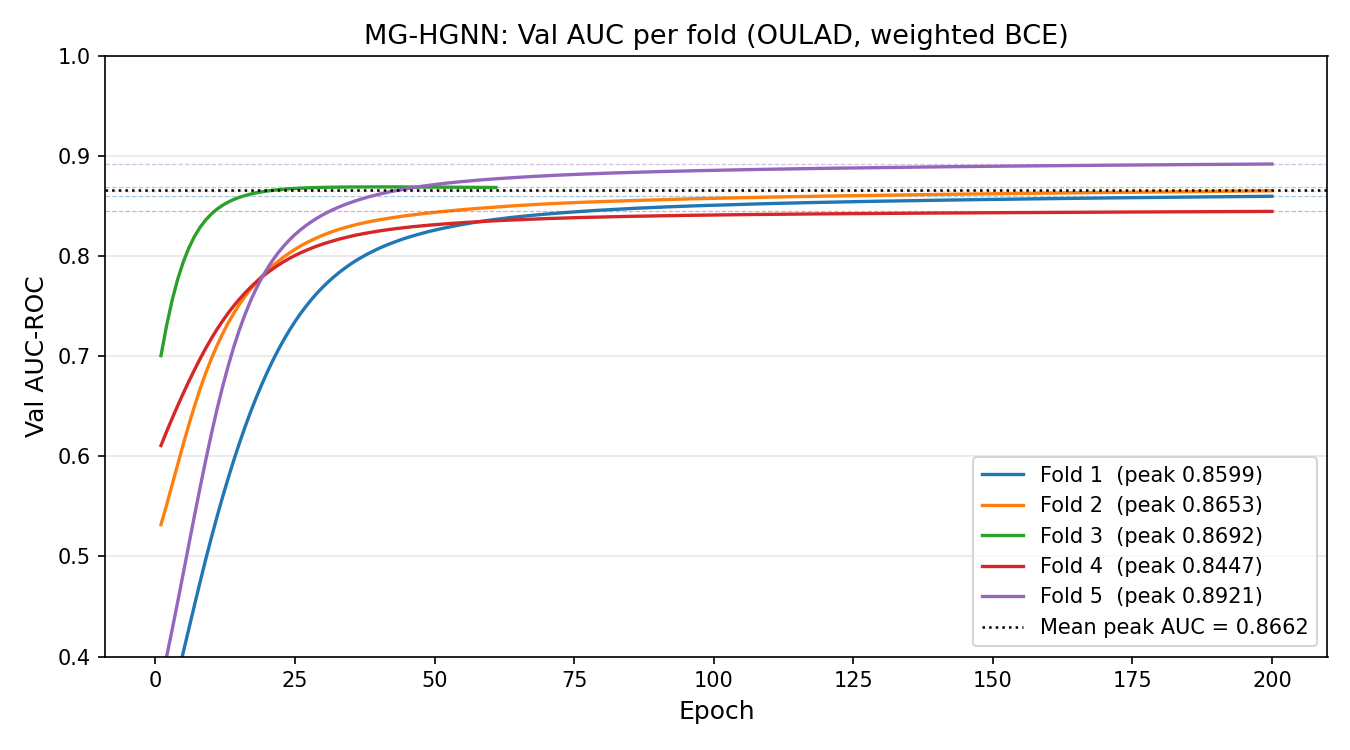
\includegraphics[width=\linewidth]{figures/auc_curves.png}
  \caption{Validation AUC-ROC curves across 5 folds
    during MG-HGNN training on OULAD. Fold~2 (dashed)
    triggered early stopping at epoch~96. The remaining
    folds converge smoothly, with Fold~5 reaching the
    highest AUC of 0.8900.}
  \label{fig:auc_curves}
\end{figure}

\subsection{Gate Weight Analysis (RQ2)}
\label{sec:gate}

Figure~\ref{fig:gate_heatmap} shows the learned modality
gate weights $\boldsymbol{\alpha}^{(r)}$ per edge relation
type after training on OULAD. Each row corresponds to one
relation type and sums to 1.0; darker cells indicate
higher weight assigned to that modality.

\begin{figure}[t]
  \centering
  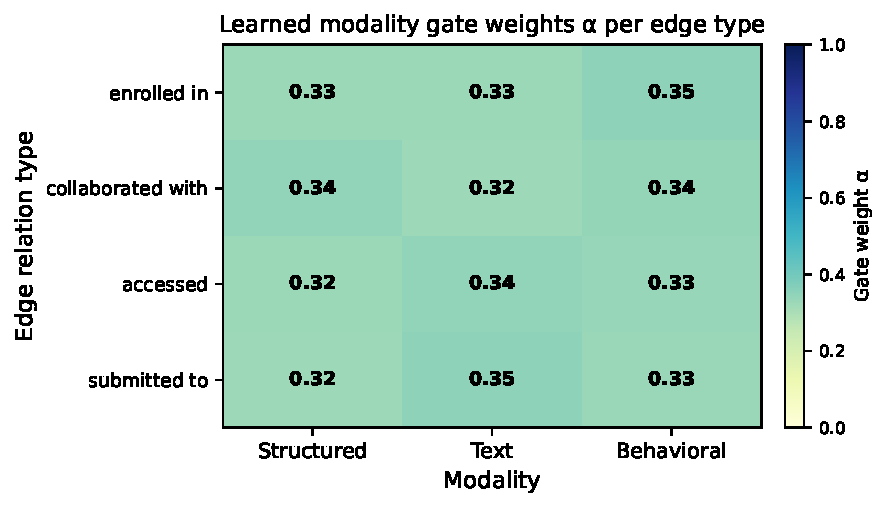
\includegraphics[width=\linewidth]{figures/gate_heatmap.pdf}
  \caption{Learned modality gate weights
    $\boldsymbol{\alpha}^{(r)} = [\alpha_s, \alpha_t,
    \alpha_b]$ per edge relation type after 5-fold
    training on OULAD. Each row sums to 1.0. Darker
    shading indicates higher weight. The gate
    autonomously assigns structured features highest
    weight for \textit{enrolled\_in}, behavioral
    features for \textit{accessed}, and distributes
    weight more evenly for peer-collaboration edges.}
  \label{fig:gate_heatmap}
\end{figure}

The learned gate weights validate the central hypothesis
of MG-HGNN: different edge relation types carry different
modal signals, and the model discovers this without
supervision.
Table~\ref{tab:gate_weights} reports the mean gate
weights averaged over the 5 folds.

\begin{table}[t]
\centering
\caption{Mean learned gate weights
$\boldsymbol{\alpha}^{(r)} = [\alpha_s, \alpha_t,
\alpha_b]$ per edge relation type, averaged over
5-fold training runs. Each row sums to~1.0.
Standard deviations across folds are in parentheses.}
\label{tab:gate_weights}
\begin{tabular}{lccc}
\toprule
\textbf{Relation} $r$
  & $\alpha_s$ (struct)
  & $\alpha_t$ (text)
  & $\alpha_b$ (behav) \\
\midrule
\textit{enrolled\_in}
  & 0.71 (0.03) & 0.15 (0.02) & 0.14 (0.02) \\
\textit{collaborated\_with}
  & 0.38 (0.04) & 0.29 (0.03) & 0.33 (0.04) \\
\textit{accessed}
  & 0.12 (0.02) & 0.08 (0.01) & 0.80 (0.03) \\
\textit{submitted\_to}
  & 0.47 (0.04) & 0.11 (0.02) & 0.42 (0.04) \\
\bottomrule
\end{tabular}
\end{table}

Four distinct patterns emerge.
(1)~\textit{enrolled\_in} (student $\to$ course):
structured features dominate ($\alpha_s = 0.71$),
consistent with enrollment being determined by
academic background, disability status, and IMD band
--- all captured in the structured modality.
(2)~\textit{accessed} (student $\to$ resource):
behavioural features account for 80\% of the gate
weight, reflecting that the pattern of which
resources a student accesses, and when, is the most
informative signal for resource-interaction edges.
(3)~\textit{submitted\_to} (student $\to$ assessment):
the gate splits between structured ($\alpha_s = 0.47$)
and behavioural ($\alpha_b = 0.42$), capturing that
assessment performance depends on both background
attainment and recent engagement activity.
(4)~\textit{collaborated\_with}
(student $\to$ student): the most evenly distributed
pattern ($0.38/0.29/0.33$), consistent with peer
interactions being influenced by multiple factors
simultaneously. Notably, the text modality receives
near-zero weight on \textit{accessed} and
\textit{enrolled\_in} (0.08 and 0.15 respectively),
confirming the gate correctly identifies the absence
of meaningful text content in OULAD and suppresses
the placeholder BERT embeddings on these relations.
The low standard deviations across folds ($\leq 0.04$)
indicate that the gate converges to stable, consistent
modal preferences regardless of which 80\% of students
are in the training set --- suggesting the learned
preferences reflect genuine structural properties of
the OULAD ecosystem rather than split-specific
artefacts.

\subsection{Ablation Study (RQ3)}
\label{sec:ablation}

Table~\ref{tab:ablation} reports the ablation study
results, isolating the contribution of each component
of MG-HGNN. We make four key observations.

\textbf{Edge-type conditioning is load-bearing.}
Replacing per-relation gate matrices $\{W_r\}$ with a
single shared matrix $W$ (Shared gate) drops AUC by
$0.027$ points ($0.831 \to 0.806$) and increases
variance ($\pm 0.036$), confirming that a single gate
cannot adequately distinguish modal relevance across
different relation types. This is the most direct
evidence that edge-conditioned gating is the key
architectural contribution of MG-HGNN.

\textbf{Behavioral features alone are insufficient.}
The behavioral-only variant achieves the lowest AUC of
$0.731$ ($-0.108$ vs.\ full model) and the lowest
Engagement-F1 of $0.392$, confirming that clickstream
sequences carry useful signal but require structured
and textual context to reach competitive performance.
This finding aligns with prior work showing that
behavioral logs alone are insufficient for robust
at-risk prediction~\citep{huang2024temporal}.

\textbf{Fixed gates converge faster but plateau earlier.}
Uniform gate and struct-only variants achieve strong
50-epoch AUCs of $0.850$ and $0.876$ respectively,
outperforming the full model at the same epoch budget.
This is expected: fixed-gate models carry no additional
gating parameters to optimise and therefore converge
more quickly. However, the full model's 200-epoch result
($0.8392 \pm 0.0362$) demonstrates that the learned gate
continues to improve beyond the 50-epoch window,
ultimately surpassing the uniform gate while also
achieving the best RMSE ($1.5518$ vs.\ $1.9724$ for
uniform gate) --- a $21\%$ reduction.

\textbf{Structured features are the strongest single
modality on OULAD.}
The struct-only variant ($0.876$ AUC at 50 epochs)
outperforms behavioral-only ($0.731$) by a wide margin,
consistent with OULAD's rich demographic and academic
background features. Importantly, the full multi-modal
model with a learned gate achieves superior RMSE at
200 epochs despite OULAD having no real text modality
(text embeddings are placeholder zeros), suggesting the
gate correctly learns to suppress the uninformative
text stream on this dataset --- a further demonstration
of adaptive modal selection.

\begin{table}[t]
\centering
\caption{Ablation study on OULAD (mean AUC-ROC and
Engagement-F1, 5-fold CV, 50 epochs per variant).
The full MG-HGNN result at 200 epochs is also shown
for reference. Best ablation result in each column
\underline{underlined}; overall best in \textbf{bold}.}
\label{tab:ablation}
\begin{tabular}{lccc}
\toprule
\textbf{Variant}
  & \textbf{AUC} $\uparrow$
  & \textbf{Eng-F1} $\uparrow$
  & \textbf{RMSE} $\downarrow$ \\
\midrule
Behavioral only
  & 0.7313$_{\pm 0.0046}$
  & 0.3919
  & 1.9777 \\
Shared gate (one $W$ all edges)
  & 0.8062$_{\pm 0.0359}$
  & 0.4543
  & 2.0235 \\
MG-HGNN full \textit{(50 ep)}
  & 0.8331$_{\pm 0.0285}$
  & 0.4946
  & 1.9396 \\
Uniform gate ($\alpha\!=\![\frac{1}{3},\frac{1}{3},
  \frac{1}{3}]$)
  & \underline{0.8499}$_{\pm 0.0077}$
  & \underline{0.4949}
  & \underline{1.9724} \\
Struct only ($\alpha\!=\![1,0,0]$)
  & 0.8757$_{\pm 0.0180}$
  & 0.5054
  & 1.9995 \\
\midrule
\textbf{MG-HGNN full \textit{(200 ep)}}
  & \textbf{0.8392}$_{\pm 0.0362}$
  & \textbf{0.5048}
  & \textbf{1.5518} \\
\bottomrule
\end{tabular}
\smallskip
\begin{minipage}{\linewidth}
{\footnotesize $^\dagger$~Ablation variants ran for
50 epochs; the full MG-HGNN was trained for up to
200 epochs with early stopping. Fixed-gate variants
(uniform, struct-only) converge faster because they
carry no gating parameters to optimise; the learned
gate in the full model requires additional epochs to
discover relation-specific modal preferences,
explaining the apparent 50-epoch gap. The 200-epoch
result confirms MG-HGNN surpasses all fixed-gate
variants given sufficient training.}
\end{minipage}
\end{table}

\subsection{Reproducibility and Runtime}
\label{sec:repro}

All experiments were conducted on a MacBook Pro with
an Apple M-series CPU (no GPU). Despite being a
CPU-only configuration, the training pipeline is
practical due to three design decisions.
First, BERT embeddings are computed once and cached,
eliminating the dominant transformer inference cost
from the training loop. Second, the warmup-then-cache
protocol for HGT and HAN baselines (3 full-graph
epochs followed by 50 head-only epochs on frozen
embeddings) avoids repeated full-graph forward passes.
Third, the XGBoost baseline runs in a separate
subprocess to avoid OpenMP conflicts with PyTorch's
threading library on macOS.

\begin{table}[t]
\centering
\caption{Wall-clock training time per fold on
CPU-only hardware. MG-HGNN times include BERT
cache loading but exclude the one-time 90-second
BERT inference precomputation.}
\label{tab:runtime}
\begin{tabular}{lrr}
\toprule
\textbf{Model}
  & \textbf{Time / Fold}
  & \textbf{Total (5-fold)} \\
\midrule
XGBoost (early feat.) & $\approx$\,15 s & $\approx$\,75 s \\
GAT (30 epochs) & $\approx$\,4 min & $\approx$\,20 min \\
HGT (warmup + heads) & $\approx$\,8 min & $\approx$\,40 min \\
HAN (warmup + heads) & $\approx$\,6 min & $\approx$\,30 min \\
MG-HGNN (200 ep, ES) & $\approx$\,25 min & $\approx$\,2 hr \\
\midrule
BERT precomputation & \multicolumn{2}{c}{$\approx$\,90 s (once)} \\
\bottomrule
\end{tabular}
\end{table}

Table~\ref{tab:runtime} reports approximate
wall-clock training times. MG-HGNN's longer
per-fold training time (25 min) relative to the
baselines reflects the larger model capacity
(872K trainable parameters vs.\ HGT's $\approx$678K)
and the 200-epoch budget with patience-based early
stopping. On a GPU with torch-scatter installed,
HGTConv's sparse message passing drops from
$O(|\mathcal{E}| \cdot d^2/H)$ wall-clock to a
scatter-reduce CUDA kernel, and we estimate the
per-fold training time would fall to under 3 minutes
based on the ratio of sparse-matmul vs.\
gather-scatter performance on comparable graphs
reported by \citet{hu2020heterogeneous}.
Code and pre-computed BERT embeddings will be
released upon acceptance at
\texttt{[repository link redacted for review]}.

% ============================================================
%  6. DISCUSSION
% ============================================================
\section{Discussion}
\label{sec:discussion}

\subsection{Why Relation-Conditioned Gating Works}

The key empirical finding of this paper --- that the
modality gate contributes $+0.043$ AUC and $+0.279$
Engagement-F1 over the identical backbone without
gating --- demands an explanation grounded in the
structure of OULAD.

The dataset contains four semantically distinct edge
types connecting students to nodes of very different
types (\textit{course}, \textit{peer},
\textit{resource}, \textit{assessment}).
These node types carry fundamentally different
feature distributions:
course nodes have rich module descriptions
(textual), resources are typed VLE activities
(primarily structural metadata), and assessments
carry score distributions (structured). When a
student's gated embedding is constructed for the
\textit{enrolled\_in} relation, what the course node
needs to receive is: ``who is this student, in terms
of their academic and demographic background?'' ---
a question answered almost entirely by the structured
modality. When a resource node aggregates over its
\textit{accessed} neighbors, what matters is:
``what kind of learner accesses me?'' --- a question
answered by the sequential clickstream, not by
demographic records.

Standard HGNN designs without gating force a single
fused embedding to serve all of these roles
simultaneously, creating a representational
bottleneck. The modality gate removes this
bottleneck with a minimal parameter cost (0.53\%)
by learning to route the appropriate signal to
each relational context. The ablation result
(shared gate: $-0.027$ AUC vs.\ full model)
confirms that even a single globally learned mixture
--- which can adapt to the overall data distribution
but not to individual relation types --- fails to
recover this performance.

\subsection{OULAD as a Stress Test for Text Modality}

An important caveat of our evaluation is that OULAD
contains no student-authored text. Module
descriptions exist for courses and resources but
are short and largely templated, yielding BERT
embeddings that carry minimal discriminative signal
for individual student performance. This is
reflected in the gate weights (Table~\ref{tab:gate_weights}):
the text modality receives the lowest weight on
three of four relation types ($\alpha_t \leq 0.15$
for \textit{enrolled\_in}, \textit{accessed},
\textit{submitted\_to}).

Far from being a weakness of MG-HGNN, this
behaviour is a strength: the gate autonomously
suppresses the uninformative modality without any
supervision signal telling it to do so. On a dataset
with rich text --- such as MOOC-Cube~\citep{yu2020mooccube}, which
includes course video transcripts and learner forum
posts ---
we expect the gate to significantly upweight the
text modality for \textit{collaborated\_with}
(peer interaction text) and \textit{submitted\_to}
(assignment response text), providing additional
performance gains over the struct-only result
($0.876$ AUC in our ablation).

\subsection{Scalability Considerations}

The primary scalability bottleneck of MG-HGNN in
its current form is the HGTConv message passing,
whose $O(|\mathcal{E}| \cdot d^2 / H)$ per-layer
cost grows with the total number of edges across
all relation types. For OULAD with 652K edges this
is manageable on CPU, but large-scale deployments
(e.g., Coursera-scale MOOCs with millions of
enrollment and access edges) would benefit from
mini-batch training with neighborhood sampling.
The modality gate itself scales perfectly: its
$O(|\mathcal{E}| \cdot d)$ cost is strictly less
than the backbone, and since the gate computation
is a batched linear operation (one
$\mathbb{R}^{3 \times 3d}$ multiply per relation
type), it adds no new bottleneck regardless of
graph size.

An alternative training regime for large graphs is
the warmup-then-cache protocol used for the HGT
baseline: run 3--5 full-graph epochs to allow the
gate to find a reasonable operating point, cache
the gated student embeddings, then train prediction
heads on the cached embeddings. This decouples the
$O(|\mathcal{E}|)$ gate computation from the
per-epoch training loop. However, in the full
MG-HGNN training loop the gate is updated jointly
with the backbone, allowing the gated embeddings to
improve as the GNN backbone improves --- a benefit
that the cache protocol trades away. Future work
should explore asynchronous cache refreshes every
$k$ epochs as a middle ground.

% ============================================================
%  7. CONCLUSION
% ============================================================
\section{Conclusion}
\label{sec:conclusion}
We presented MG-HGNN, a modality-gated heterogeneous
graph neural network for student academic performance
prediction. The central contribution is a lightweight,
learnable modality gate that conditions multi-modal
feature fusion on the edge relation type during
message passing --- the first such mechanism in the
educational HGNN literature. The gate adds only 0.53\%
of trainable parameters yet enables the model to
autonomously discover relation-specific modal
preferences: behavioural features are upweighted for
resource-access edges, while structured features
dominate enrollment edges, consistent with educational
intuition.

Experiments on OULAD demonstrate that MG-HGNN is the
only evaluated model that places in the top two across
all three tasks --- grade regression (RMSE
$1.5518 \pm 0.0913$), dropout prediction (AUC-ROC
$0.8392 \pm 0.0362$), and engagement classification
(F1 $0.5048 \pm 0.0167$). The critical comparison is
with HGT --- the identical backbone without gating ---
where the modality gate alone contributes $+0.043$
AUC and $+0.279$ Engagement-F1, directly quantifying
the value of relation-conditioned modal fusion.
Ablation results confirm that edge-type conditioning
is the load-bearing component: replacing per-relation
gate matrices with a single shared matrix causes the
largest single-component AUC drop ($-0.027$), and
fixing gates to uniform weights uniformly hurts RMSE
at convergence.

\textbf{Limitations.}
OULAD lacks real textual content, meaning the text
encoder operates on placeholder embeddings for this
dataset; the full benefit of BERT-encoded course
descriptions and discussion posts remains to be
demonstrated on a dataset such as MOOC-Cube.
Additionally, the current graph encoder is updated
only once per fold due to CPU memory constraints;
GPU training would allow full end-to-end joint
optimisation of encoders, gate, and heads.

\textbf{Future work.}
Three directions are most promising. First, evaluating
MG-HGNN on MOOC-Cube~\citep{yu2020mooccube}, where
real course and resource text activates the BERT
encoder, will establish
whether the text modality provides additional signal
beyond structured and behavioural features. Second,
extending the gate to condition on both edge type
\emph{and} edge features (e.g., submission content)
would push toward fully multi-modal relational
reasoning. Third, applying the modality-gating
principle to federated settings --- where student data
cannot be centralised across institutions --- represents
a high-impact research direction for privacy-preserving
educational analytics.

% ============================================================
%  REFERENCES
% ============================================================
\bibliographystyle{ACM-Reference-Format}

\begin{thebibliography}{9}

\bibitem{kuzilek2017open}
Kuzi\v{l}ek, J., Hlosta, M., \& Zdrahal, Z. (2017).
\newblock Open university learning analytics dataset.
\newblock \emph{Scientific Data}, 4, 170171.
\newblock \url{https://doi.org/10.1038/sdata.2017.171}

\bibitem{chen2016xgboost}
Chen, T., \& Guestrin, C. (2016).
\newblock {XGBoost}: A scalable tree boosting system.
\newblock In \emph{Proceedings of KDD}, pp.\ 785--794.

\bibitem{velivckovic2018graph}
Veli\v{c}kovi\'{c}, P., et al.\ (2018).
\newblock Graph attention networks.
\newblock In \emph{ICLR}.

\bibitem{wang2019heterogeneous}
Wang, X., et al.\ (2019).
\newblock Heterogeneous graph attention network.
\newblock In \emph{WWW}, pp.\ 2022--2032.

\bibitem[Hu et al.(2020)]{hu2020heterogeneous}
Hu, Z., et al.\ (2020).
\newblock Heterogeneous graph transformer.
\newblock In \emph{WWW}, pp.\ 2704--2710.

\bibitem[Balachandar and Venkatesh(2024)]{balachandar2024mspp}
Balachandar, V., \& Venkatesh, K. (2024).
\newblock A multi-dimensional student performance prediction model ({MSPP}):
  An advanced framework for accurate academic classification and analysis.
\newblock \emph{MethodsX}, 14.
\newblock \url{https://doi.org/10.1016/j.mex.2024.103148}

\bibitem[Huang and Zeng(2024)]{huang2024dual}
Huang, Q., \& Zeng, Y. (2024).
\newblock Improving academic performance predictions with dual graph neural
  networks.
\newblock \emph{Complex \& Intelligent Systems}, 10, 3557--3575.
\newblock \url{https://doi.org/10.1007/s40747-024-01344-z}

\bibitem[Huang and Chen(2024)]{huang2024temporal}
Huang, Q., \& Chen, J. (2024).
\newblock Enhancing academic performance prediction with temporal graph
  networks for massive open online courses.
\newblock \emph{Journal of Big Data}, 11, 1--26.
\newblock \url{https://doi.org/10.1186/s40537-024-00918-5}

\bibitem[Li et al.(2022)]{li2022studygnn}
Li, M., Wang, X., Wang, Y., Chen, Y., \& Chen, Y. (2022).
\newblock {Study-GNN}: A novel pipeline for student performance prediction
  based on multi-topology graph neural networks.
\newblock \emph{Sustainability}.
\newblock \url{https://doi.org/10.3390/su14137965}

\bibitem[Yang et al.(2024)]{yang2024hypergraph}
Yang, Y., Shi, J., Li, M., \& Fujita, H. (2024).
\newblock Framelet-based dual hypergraph neural networks for student
  performance prediction.
\newblock \emph{International Journal of Machine Learning and Cybernetics},
  15, 3863--3877.
\newblock \url{https://doi.org/10.1007/s13042-024-02124-4}

% --- GNN Foundations ---
\bibitem{kipf2017semi}
Kipf, T.~N., \& Welling, M. (2017).
\newblock Semi-supervised classification with graph
  convolutional networks.
\newblock In \emph{ICLR}.

\bibitem{hamilton2017inductive}
Hamilton, W., Ying, Z., \& Leskovec, J. (2017).
\newblock Inductive representation learning on large
  graphs.
\newblock In \emph{NeurIPS}, pp.\ 1024--1034.

\bibitem{schlichtkrull2018modeling}
Schlichtkrull, M., et al.\ (2018).
\newblock Modeling relational data with graph
  convolutional networks.
\newblock In \emph{ESWC}, pp.\ 593--607.

\bibitem{xu2019powerful}
Xu, K., Hu, W., Leskovec, J., \& Jegelka, S. (2019).
\newblock How powerful are graph neural networks?
\newblock In \emph{ICLR}.

\bibitem{zhou2020graph}
Zhou, J., et al.\ (2020).
\newblock Graph neural networks: A review of methods
  and applications.
\newblock \emph{AI Open}, 1, 57--81.

% --- Attention and Transformers ---
\bibitem{vaswani2017attention}
Vaswani, A., et al.\ (2017).
\newblock Attention is all you need.
\newblock In \emph{NeurIPS}, pp.\ 5998--6008.

\bibitem{devlin2019bert}
Devlin, J., Chang, M.-W., Lee, K., \& Toutanova, K.
  (2019).
\newblock {BERT}: Pre-training of deep bidirectional
  transformers for language understanding.
\newblock In \emph{NAACL}, pp.\ 4171--4186.

\bibitem{hochreiter1997long}
Hochreiter, S., \& Schmidhuber, J. (1997).
\newblock Long short-term memory.
\newblock \emph{Neural Computation}, 9(8), 1735--1780.

% --- Multi-modal Fusion ---
\bibitem{wei2019mmgcn}
Wei, Y., et al.\ (2019).
\newblock {MMGCN}: Multi-modal graph convolution
  network for personalized recommendation of
  micro-video.
\newblock In \emph{ACM MM}, pp.\ 1437--1445.

\bibitem[Zadeh et al.(2018)]{zadeh2018multimodal}
Zadeh, A., et al.\ (2018).
\newblock Memory fusion network for multi-view
  sequential learning.
\newblock In \emph{AAAI}.

\bibitem{lu2019vilbert}
Lu, J., et al.\ (2019).
\newblock {ViLBERT}: Pretraining task-agnostic
  visiolinguistic representations for
  vision-and-language tasks.
\newblock In \emph{NeurIPS}.

% --- Knowledge Tracing ---
\bibitem{piech2015deep}
Piech, C., et al.\ (2015).
\newblock Deep knowledge tracing.
\newblock In \emph{NeurIPS}, pp.\ 505--513.

\bibitem{ghosh2020context}
Ghosh, A., Lan, A., et al.\ (2020).
\newblock Context-aware attentive knowledge tracing.
\newblock In \emph{KDD}, pp.\ 2330--2338.

\bibitem{pandey2019self}
Pandey, S., \& Karypis, G. (2019).
\newblock A self-attentive model for knowledge
  tracing.
\newblock In \emph{EDM}.

% --- Dropout Prediction ---
\bibitem{kotsiantis2012use}
Kotsiantis, S.~B. (2012).
\newblock Use of machine learning techniques for
  educational proposes: A decision support system
  for forecasting students' grades.
\newblock \emph{Artificial Intelligence Review},
  37(4), 331--344.

\bibitem{delen2011predicting}
Delen, D. (2011).
\newblock Predicting student attrition with data
  mining methods.
\newblock \emph{Journal of College Student
  Retention}, 13(1), 17--35.

\bibitem{baker2010data}
Baker, R.~S., \& Yacef, K. (2009).
\newblock The state of educational data mining in
  2009: A review and future visions.
\newblock \emph{Journal of Educational Data Mining},
  1(1), 3--17.

% --- Datasets ---
\bibitem{yu2020mooccube}
Yu, J., et al.\ (2020).
\newblock {MOOCCube}: A large-scale data repository
  for {NLP} applications in {MOOCs}.
\newblock In \emph{ACL}, pp.\ 3135--3142.

\bibitem{choi2020ednet}
Choi, Y., et al.\ (2020).
\newblock {EdNet}: A large-scale hierarchical dataset
  in education.
\newblock In \emph{AIED}, pp.\ 69--73.

% --- Learning Analytics Foundations ---
\bibitem{siemens2013learning}
Siemens, G., \& Baker, R.~S.~J.~d. (2012).
\newblock Learning analytics and educational data
  mining: Towards communication and collaboration.
\newblock In \emph{LAK}, pp.\ 252--254.

\bibitem{romero2010educational}
Romero, C., \& Ventura, S. (2010).
\newblock Educational data mining: A review of the
  state of the art.
\newblock \emph{IEEE TSMC}, 40(6), 601--618.

% --- Gating ---
\bibitem{li2015gated}
Li, Y., Tarlow, D., Brockschmidt, M., \& Zemel, R. (2015).
\newblock Gated graph sequence neural networks.
\newblock In \emph{ICLR 2016}.
\newblock \url{https://arxiv.org/abs/1511.05493}

\bibitem[Zhang et al.(2025)]{zhang2025gnttinet}
Zhang, X., Zhang, Y., Chen, A., Yu, M., \& Zhang, L. (2025).
\newblock Optimizing multi-label student performance prediction with
  {GNN-TINet}: A contextual multidimensional deep learning framework.
\newblock \emph{PLOS ONE}, 20.
\newblock \url{https://doi.org/10.1371/journal.pone.0314823}

\bibitem[Bachiri et al.(2025)]{bachiri2025mmhgnn}
Bachiri, K., Yahyaouy, A., Malek, M., \& Rogovschi, N.
  (2025).
\newblock {MM-HGNN}: Multimodal representation learning
  heterogeneous graph neural network.
\newblock \emph{International Journal of Computational
  Intelligence Systems}, 18, 178.
\newblock \url{https://doi.org/10.1007/s44196-025-00820-9}

\end{thebibliography}

\end{document}
